\chapter{Implementacja}

\section{Architektura}

%TODO zarys architektóry


%TODO Rozdział do przebudowy

%TODO Struktura REST


\section{Aplikacja serwerowa}
Do zarządzania danymi wykorzystywana jest aplikacja serwerowa. Przetwarza ona żądania aplikacji klienckiej. Dostarcza ona funkcjonalność uwierzytelniania i autoryzacji. W wyniku zapytań wysłanych przez aplikację kliencką wyświetlane są w aplikacji odpowiednie dane. Można też dodawać i usuwać odpowiednie rekordy. Implementacja odbywa się z wykorzystaniem biblioteki Spring oraz języku Java. Do mapowania obiektowo-relacyjnego wykorzystany jest hibernate.

\subsection{Struktura projektu}
Ścieżka pakietowa wykorzystana jest odwróconą ścieżką domenową Politechniki Wrocławskiej oraz nazwy projektu: pl.pwr.edu.computermanagamenttool. Następnie pakiety które są dołączone do tej ścieżki odpowiadają funkcjom któe pełnią klasy. Wyróżnia się tutaj:

\begin{itemize}[label=•]
\item controller - pakiet który grupuje klasy kontrolerów. Kontrolery są odpowiedzialne za obsługę żądań HTTP, zarządzanie przekazywaniem danych między modelem a widokiem oraz sterowanie logiką aplikacji. Kontroler definiuje metody obsługujące różne ścieżki URL i żądania HTTP.
\item entity - pakiet grupujący encje które reprezentują obiekty przechowywane w bazie danych. Każda encja mapuje się na tabelę w bazie danych, a pola encji odpowiadają kolumną w tej tabeli. Do mapowania obiektowo relacyjnego wykorzystano framework Hibernate.
\item repository - pakiet który zawiera repozytoria służące do komunikacji z bazą danych. Spring Data JPA umożliwia definiowanie interfejsów, a implementacje dostarcza automatycznie na podstawie nazw metod.
\item service - pakiet grupujący klasy które odpowiadają za logikę biznesową. Są odpowiedzialne za przetwarzanie danych, wykonywanie operacji i kordynacje działań między kontrolerami a repozytoriami. Serwisy wywoływane są przez kontrolery
\end{itemize}


\begin{figure}[h]
    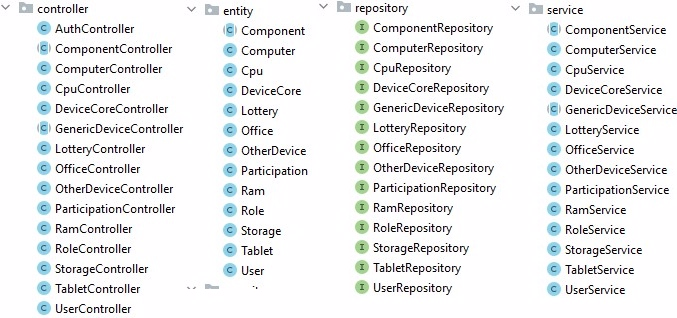
\includegraphics[scale=1.0]{rys05/pakiety.jpg}
    \caption{Pakiety w strukturze projektu}
    \label{pakiety_etykieta}
\end{figure}

\newpage
\subsection {Encja z wykorzystaniem Hibernate}

W diagramie encji Rys. \ref{ErDiagram_etykieta} istnieją 4 klasy odpowiedzialne za sprzęt komputerowy. Klasa nadrzędna device\_core oraz klasy potomne: other\_device, tablet, computer. Klasy potomne posiadają wszystkie atrybuty które posiada klasa nadrzędna. System pozwala na wykonanie zapytania które pobierze dane wszystkich dostępnych urządzeń niezależnie od typu. Wykorzystano tutaj mechanizm dziedziczenia dostarczany przez Hibernate: TABLE\_PER\_CLASS.

\begin{lstlisting}[language=Java, style=JavaStyle, caption={Fragment klasy nadrzędnej DeviceCore}, label={entity_deviceCore}]
@Entity
@Table(name = "device_core")
@Inheritance(strategy = InheritanceType.TABLE_PER_CLASS)
public class DeviceCore {
    @Id
    @GeneratedValue(strategy = GenerationType.TABLE)
    @Column(name = "id", nullable = false)
    private Integer id;

    @Column(name = "device_type", length = 50)
    private String deviceType;

    @Column(name = "device_name", length = 50)
    private String deviceName;

\end{lstlisting}

Wykorzystana w listingu \ref{entity_deviceCore} w linii 3 strategia InheritanceType.TABLE\_PER\_CLASS sprawia że każda klasa dziedzicząca ma swoją własną tabelę  w bazie danych. Oznacza to że dla każdej klasy w hierarchii dziedziczenia utworzona zostanie oddzielna tabela w bazie danych, a tableta ta zawierać będzie zarówno pola z tej klasy jak i nadklasy. Dodatkowo wszystkie rekordy klas potomnych z baz danych zawierać będą unikalne indeksy w odniesieniu do innych klas potomnych.

\begin{lstlisting}[language=Java, style=JavaStyle,  caption={Fragment klasy potomnej Computer}, label={entity_computer}]
@Entity
@Table(name = "computer")
public class Computer extends DeviceCore{

    public static final String DEVICE_TYPE = "COMPUTER";
    @Column(name = "serial_number", length = 50)
    private String serialNumber;

    @Column(name = "operating_system", length = 50)
    private String operatingSystem;

    @Column(name = "battery_life", length = 50)
    private String batteryLife;
		
		@ManyToOne(fetch = FetchType.EAGER)
    @JoinColumn(name = "cpu_id")
    private Cpu cpu;

\end{lstlisting}

Zdefiniowana klasa opisana w powyższym Listingu \ref{entity_computer} dodaje nowe pola do tabeli rozszerzjąc funkcjonalność encji. Zmienna statyczna zdefiniowana w linii 5 jest pomocniczą zmienną na podstawie której można określić jaki typ klasy reprezentuje dany obiekt co ułatwi zarządzanie żądaniami w aplikacji klienckiej.

\subsection{Repozytorium}
Repozytorium sprzętu komputerowego zostało napisane z użyciem wyrażeń generycznych. Wykorzystanie ich przyczynia się do uproszczenia kodu oraz łatwiejszej jego rozbudowy.

\begin{lstlisting}[language=Java, style=JavaStyle,  caption={Generyczne repozytorium sprzętu komputerowego}, label={repo_genericDevice}]
@NoRepositoryBean
public interface GenericDeviceRepository<T extends DeviceCore> extends JpaRepository<T, Integer> {

    List<T> findAllByReadyToSellIsTrue();
    List<T> findAllByReadyToSellIsFalse();
    List<T> findAllByOfficeId(int officeId);
}
\end{lstlisting}

W lini 1 adnotacja @NoRepositoryBean jest używana do oznaczenia interfejsów które nie mają mieć swojej instancji. Oznacza to, że nie jest on przeznaczony do utworzenia instancji repozytorium w trakcie uruchomiania aplikacji. Z racji tego że klasy sprzętu komputerowego mają zbliżone funkcjonalności nie trzeba dostarczać tych samych interfejsów we wszystkich repozytoriach tylko zastosować schemat dziedziczenia. To samo dotyczy się kontrolerów co pokazano w następnym podrozdziale.

\subsection{Kontroler sprzętu komputerowego}

\begin{lstlisting}[language=Java, style=JavaStyle,  caption={Wybrane metody generycznego kontrolera sprzętu komputerowego}, label={controller_genericDevice}]
@GetMapping("/all")
 List<T> getAllBasicDevices(){
 return genericDeviceService.getAllDevices();
} 
@DeleteMapping("/{id}")
void deleteDevice(@PathVariable int id){
genericDeviceService.deleteDevice(id);
}
\end{lstlisting}

Powyższy Listing kodu \ref{repo_genericDevice} umożliwia jednym zapytaniem uzyskanie wszystkich danych dotyczące urządzeń, wliczając to także dane które są unikalne dla klas potomnych. Dzięki temu można zestawić w tabeli a aplikacji klienckiej ogólne informacje dotyczące sprzętu. Zastosowano mechanizm dziedziczenia, dzięki czemu klasy dziedziczące po generycznym repozytorium umożliwiają uzyskanie tylko danych sprzętów należących do kategorii klasy potomnych. Aby uzyskać właśnie tylko sprzęty klasy potomnej wystarczy zmienić tylko endpoint i nie jest konieczne powielanie kodu. Klasy dziedziczące rozszerzają funkcjonalność generycznego repozytorium dodając metody unikalne dla wybranego sprzętu.

\subsection{Dodawanie komputera z wykorzystaniem klasy nadrzędnej}
Wszystkie klasy potomne mają wspólne atrybuty dlatego wykorzystano generyczny serwis by zredukować powielenie kodu

\begin{lstlisting}[language=Java, style=JavaStyle,  caption={Dodawanie Tabletu z wykorzystaniem klasy nadrzędnej}, label={service_tablet}]
protected DeviceCore addDevice(Class<? extends DeviceCore> deviceClass, String deviceName, Double price, String description, Integer age, Boolean readyToSell, Integer officeId) {

        if(officeId == null){
            throw new RuntimeException("Office required");
        }
        Optional<Office> officeOptional = officeRepository.findById(officeId);
        Office office = officeOptional.orElseThrow(() -> new RuntimeException("Office not found with id: " + officeId));

        DeviceCore deviceCore;
        try {
            deviceCore = deviceClass.getDeclaredConstructor().newInstance();
        } catch (InstantiationException | IllegalAccessException | NoSuchMethodException | InvocationTargetException e) {
            throw new RuntimeException("Error creating device", e);
        }

        deviceCore.setDeviceName(deviceName);
        deviceCore.setPrice(price);
        deviceCore.setDescription(description);
        deviceCore.setAge(age);
        deviceCore.setReadyToSell(readyToSell);
        deviceCore.setOffice(office);

        return deviceCore;
    }

public Tablet addTablet(String deviceName, Double price, String description,
                            Integer age, Boolean readyToSell, Integer officeId,
                            String screenSize, String operatingSystem, String batteryLife){

        Tablet tablet = (Tablet) addDevice(Tablet.class, deviceName, price, description,
                                                                age, readyToSell, officeId);

        tablet.setScreenSize(screenSize);
        tablet.setOperatingSystem(operatingSystem);
        tablet.setBatteryLife(batteryLife);

        return genericDeviceRepository.save(tablet);
    }

\end{lstlisting}

W Listingu \ref{service_tablet} metoda w linii 1 z klasy generycznej oprócz atrybutów pól przyjmuję też jako argument obiekt typu Class. Wykorzystywany jest on w linii 11 do stworzenia instancji klasy. Dzięki temu we wszystkich klasach potomnych, wspólne atrybuty są ustawiane przez klasę nadrzędną(linie 16-21). Przykład ustawiania unikalnych pól klasy podrzędnej są w liniach 33-35.

\section {Aplikacja kliencka}